\section{Arquitetura do Sistema}
\frame
{
\frametitle{Módulos do Sistema}
Divisão do código em 4 módulos visando o desenvolvimento distribuído:
\begin{itemize}
\item \emph{Core}
\item \emph{GTFS Importer}
\item \emph{Web Service}
\item Cliente
\end{itemize}
}

\frame
{
\frametitle{Visão geral do sistema}
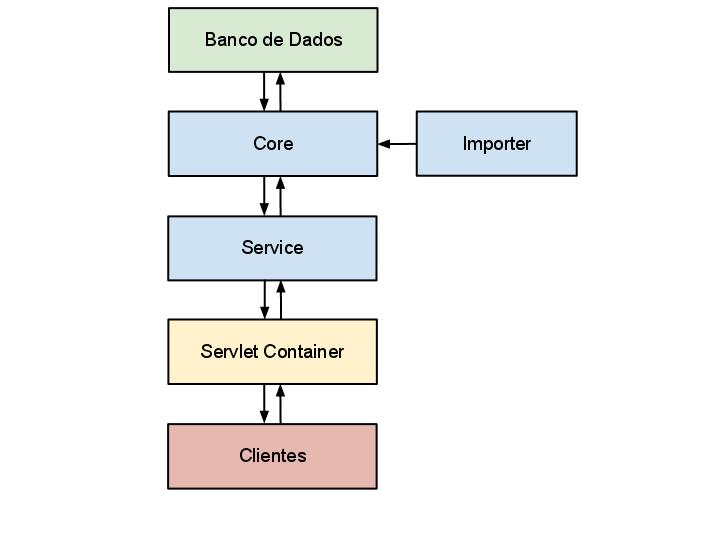
\includegraphics[width=1\textwidth]{./imgs/arquitetura.png}
}

\subsection{Core}
\frame
{
\frametitle{\emph{Core}}
Contém as representações das entidades do sistema.
\begin{itemize}
\item Vértices
\item Relações
\end{itemize}
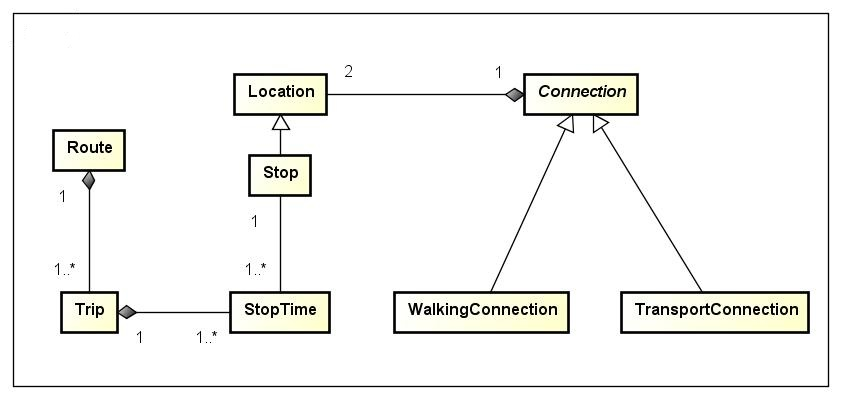
\includegraphics[width=1\textwidth]{./imgs/CoreDiagram.png}
}

\frame
{
\frametitle{\emph{Factories}}
Interface para criação de entidades do \emph{Core}.
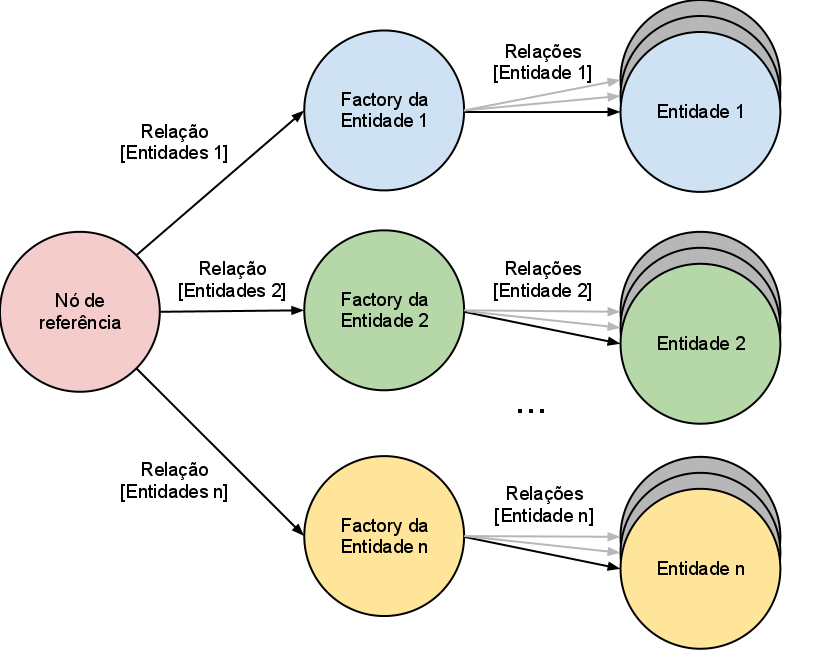
\includegraphics[width=0.8\textwidth]{./imgs/grafoFactory.png}
}

\frame
{
\frametitle{\emph{DatabaseController}}
Interface para centralizar o acesso ao banco de dados.
\begin{itemize}
\item Inicia e finaliza transações.
\item Abstração da conexão entre sistema e BD.
\end{itemize}
}


